\documentclass[10pt]{article}
\usepackage[utf8]{inputenc}
\usepackage[margin=0in,paperwidth=12in,paperheight=4in]{geometry}
\usepackage{tikz}
\usepackage{xcolor}
\usepackage{amsmath,amssymb}
\usetikzlibrary{shapes.geometric, arrows.meta, positioning, calc, backgrounds}
\pagestyle{empty}

\definecolor{bgdark}{HTML}{0F172A}
\definecolor{cardbg}{HTML}{1E293B}
\definecolor{bordercol}{HTML}{334155}
\definecolor{accentblue}{HTML}{38BDF8}
\definecolor{accentgreen}{HTML}{10B981}
\definecolor{accentorange}{HTML}{F59E0B}
\definecolor{accentpurple}{HTML}{A855F7}
\definecolor{accentred}{HTML}{EF4444}
\definecolor{accentcyan}{HTML}{06B6D4}
\definecolor{textwhite}{HTML}{F8FAFC}
\definecolor{textmuted}{HTML}{94A3B8}

\begin{document}
\noindent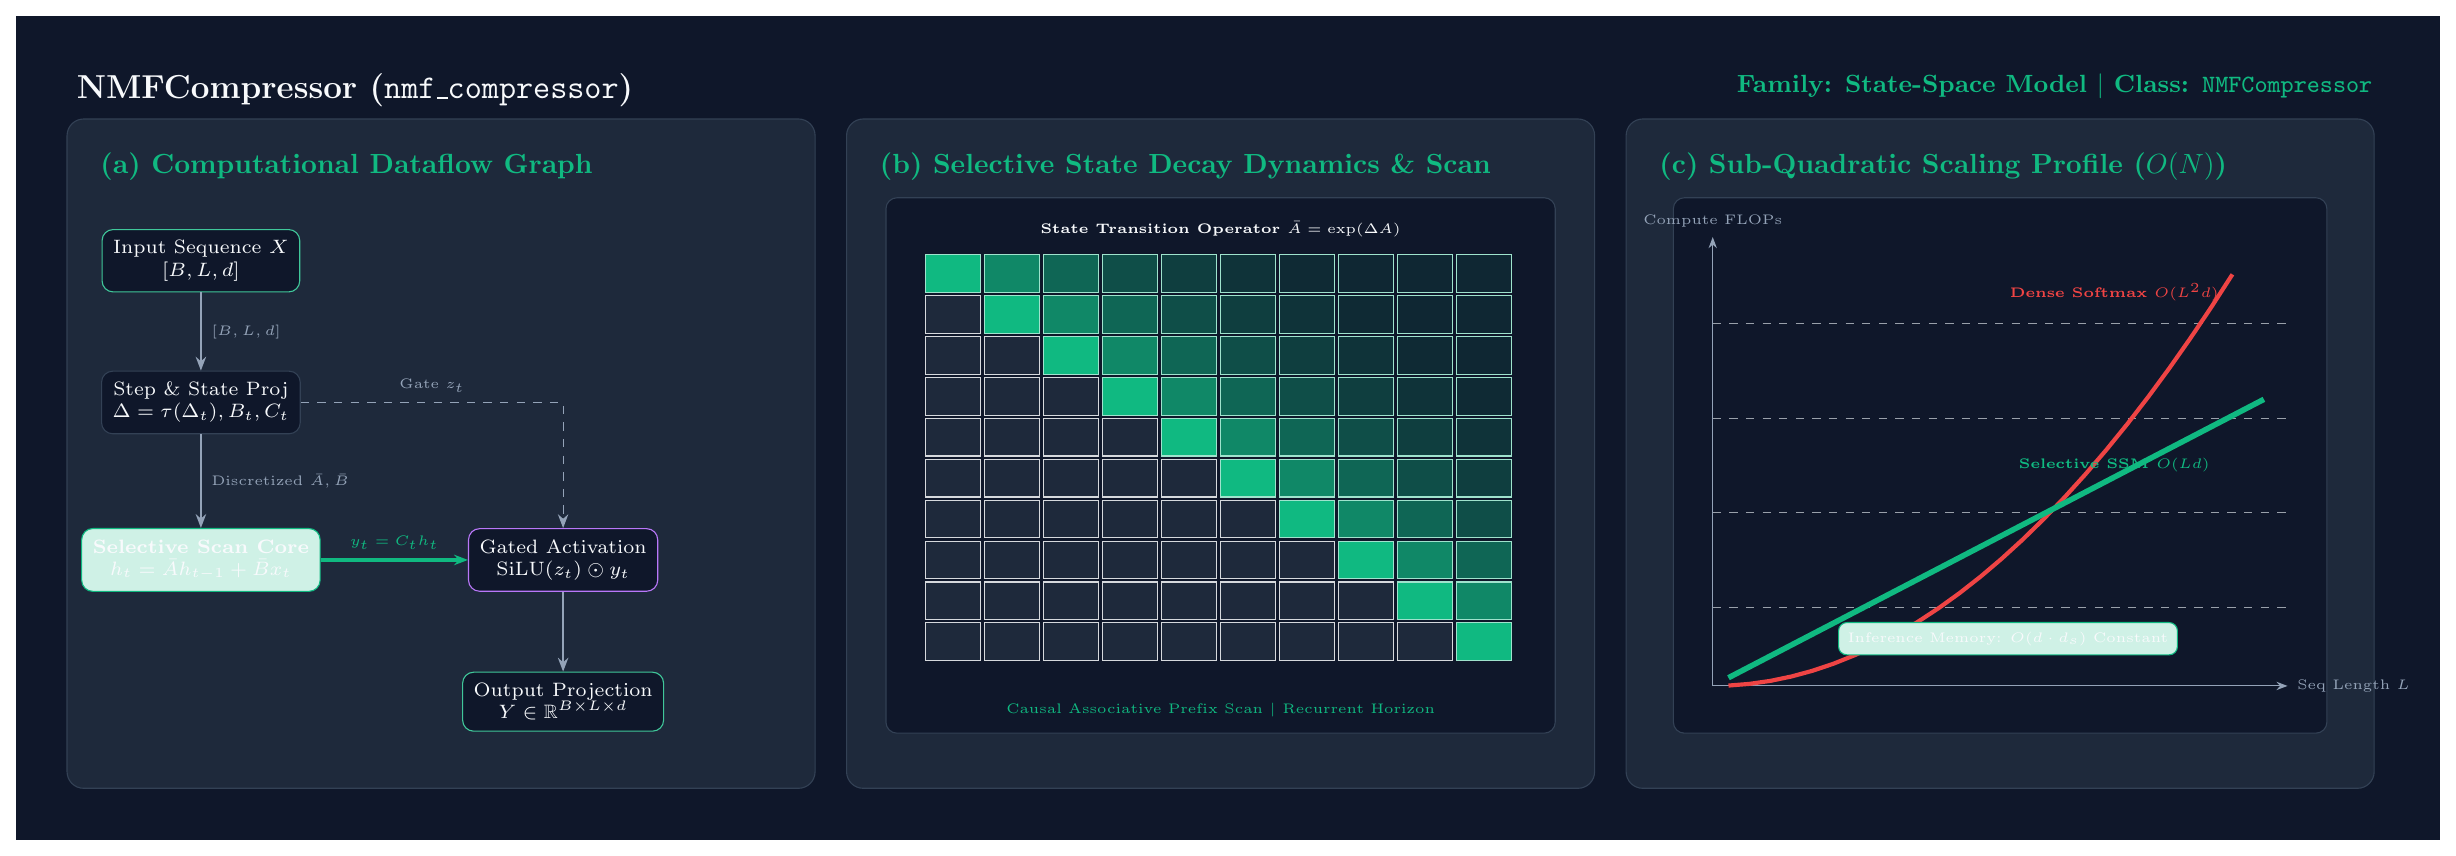
\begin{tikzpicture}[
    background rectangle/.style={fill=bgdark}, show background rectangle,
    scale=1.0, every node/.style={transform shape}
]

\clip (0,0) rectangle (30.48, 10.16);

% Title Header
\node[anchor=north west, text=textwhite, font=\large\bfseries] at (0.5, 9.7) {NMFCompressor (\texttt{nmf\_compressor})};
\node[anchor=north east, text=accentgreen, font=\small\bfseries] at (29.9, 9.7) {Family: State-Space Model $\mid$ Class: \texttt{NMFCompressor}};

% Panel A: Computational Architecture
\draw[fill=cardbg, draw=bordercol, rounded corners=6pt] (0.5, 0.5) rectangle (10.0, 9.0);
\node[anchor=north west, text=accentgreen, font=\bfseries\normalsize] at (0.8, 8.7) {(a) Computational Dataflow Graph};

\node[draw=accentgreen!80, fill=bgdark, rounded corners=4pt, text=textwhite, font=\scriptsize, align=center, inner sep=4pt] (inp) at (2.2, 7.2) {Input Sequence $X$\\$[B, L, d]$};
\node[draw=bordercol, fill=bgdark, rounded corners=4pt, text=textwhite, font=\scriptsize, align=center, inner sep=4pt] (proj) at (2.2, 5.4) {Step \& State Proj\\$\Delta = \tau(\Delta_t), B_t, C_t$};
\node[draw=accentgreen, fill=accentgreen!20, rounded corners=4pt, text=textwhite, font=\scriptsize\bfseries, align=center, inner sep=4pt] (core) at (2.2, 3.4) {Selective Scan Core\\$h_t = \bar{A} h_{t-1} + \bar{B} x_t$};
\node[draw=accentpurple!80, fill=bgdark, rounded corners=4pt, text=textwhite, font=\scriptsize, align=center, inner sep=4pt] (gate) at (6.8, 3.4) {Gated Activation\\$\mathrm{SiLU}(z_t) \odot y_t$};
\node[draw=accentgreen!80, fill=bgdark, rounded corners=4pt, text=textwhite, font=\scriptsize, align=center, inner sep=4pt] (outp) at (6.8, 1.6) {Output Projection\\$Y \in \mathbb{R}^{B \times L \times d}$};

        \draw[-{Stealth[length=5pt]}, textmuted, line width=1pt] (inp) -- (proj) node[midway, right, font=\tiny] {$[B, L, d]$};
        \draw[-{Stealth[length=5pt]}, textmuted, line width=1pt] (proj) -- (core) node[midway, right, font=\tiny] {Discretized $\bar{A}, \bar{B}$};
        \draw[-{Stealth[length=5pt]}, accentgreen, line width=1.2pt] (core) -- (gate) node[midway, above, text=accentgreen, font=\tiny] {$y_t = C_t h_t$};
        \draw[-{Stealth[length=5pt]}, textmuted, line width=1pt] (gate) -- (outp);
        \draw[-{Stealth[length=5pt]}, dashed, textmuted] (proj) -| (gate) node[pos=0.25, above, font=\tiny] {Gate $z_t$};
        

% Panel B: Structural Pattern & Dynamics
\draw[fill=cardbg, draw=bordercol, rounded corners=6pt] (10.4, 0.5) rectangle (19.9, 9.0);
\node[anchor=north west, text=accentgreen, font=\bfseries\normalsize] at (10.7, 8.7) {(b) Selective State Decay Dynamics \& Scan};
\draw[draw=bordercol, fill=bgdark, rounded corners=4pt] (10.9, 1.2) rectangle (19.4, 8.0);
\node[text=textwhite, font=\tiny\bfseries] at (15.15, 7.6) {State Transition Operator $\bar{A} = \exp(\Delta A)$};
\draw[fill=accentgreen!100!bgdark, draw=accentgreen!40] (11.40, 6.80) rectangle (12.10, 7.28);
\draw[fill=cardbg, draw=bordercol!20] (11.40, 6.28) rectangle (12.10, 6.76);
\draw[fill=cardbg, draw=bordercol!20] (11.40, 5.76) rectangle (12.10, 6.24);
\draw[fill=cardbg, draw=bordercol!20] (11.40, 5.24) rectangle (12.10, 5.72);
\draw[fill=cardbg, draw=bordercol!20] (11.40, 4.72) rectangle (12.10, 5.20);
\draw[fill=cardbg, draw=bordercol!20] (11.40, 4.20) rectangle (12.10, 4.68);
\draw[fill=cardbg, draw=bordercol!20] (11.40, 3.68) rectangle (12.10, 4.16);
\draw[fill=cardbg, draw=bordercol!20] (11.40, 3.16) rectangle (12.10, 3.64);
\draw[fill=cardbg, draw=bordercol!20] (11.40, 2.64) rectangle (12.10, 3.12);
\draw[fill=cardbg, draw=bordercol!20] (11.40, 2.12) rectangle (12.10, 2.60);
\draw[fill=accentgreen!70!bgdark, draw=accentgreen!40] (12.15, 6.80) rectangle (12.85, 7.28);
\draw[fill=accentgreen!100!bgdark, draw=accentgreen!40] (12.15, 6.28) rectangle (12.85, 6.76);
\draw[fill=cardbg, draw=bordercol!20] (12.15, 5.76) rectangle (12.85, 6.24);
\draw[fill=cardbg, draw=bordercol!20] (12.15, 5.24) rectangle (12.85, 5.72);
\draw[fill=cardbg, draw=bordercol!20] (12.15, 4.72) rectangle (12.85, 5.20);
\draw[fill=cardbg, draw=bordercol!20] (12.15, 4.20) rectangle (12.85, 4.68);
\draw[fill=cardbg, draw=bordercol!20] (12.15, 3.68) rectangle (12.85, 4.16);
\draw[fill=cardbg, draw=bordercol!20] (12.15, 3.16) rectangle (12.85, 3.64);
\draw[fill=cardbg, draw=bordercol!20] (12.15, 2.64) rectangle (12.85, 3.12);
\draw[fill=cardbg, draw=bordercol!20] (12.15, 2.12) rectangle (12.85, 2.60);
\draw[fill=accentgreen!49!bgdark, draw=accentgreen!40] (12.90, 6.80) rectangle (13.60, 7.28);
\draw[fill=accentgreen!70!bgdark, draw=accentgreen!40] (12.90, 6.28) rectangle (13.60, 6.76);
\draw[fill=accentgreen!100!bgdark, draw=accentgreen!40] (12.90, 5.76) rectangle (13.60, 6.24);
\draw[fill=cardbg, draw=bordercol!20] (12.90, 5.24) rectangle (13.60, 5.72);
\draw[fill=cardbg, draw=bordercol!20] (12.90, 4.72) rectangle (13.60, 5.20);
\draw[fill=cardbg, draw=bordercol!20] (12.90, 4.20) rectangle (13.60, 4.68);
\draw[fill=cardbg, draw=bordercol!20] (12.90, 3.68) rectangle (13.60, 4.16);
\draw[fill=cardbg, draw=bordercol!20] (12.90, 3.16) rectangle (13.60, 3.64);
\draw[fill=cardbg, draw=bordercol!20] (12.90, 2.64) rectangle (13.60, 3.12);
\draw[fill=cardbg, draw=bordercol!20] (12.90, 2.12) rectangle (13.60, 2.60);
\draw[fill=accentgreen!34!bgdark, draw=accentgreen!40] (13.65, 6.80) rectangle (14.35, 7.28);
\draw[fill=accentgreen!49!bgdark, draw=accentgreen!40] (13.65, 6.28) rectangle (14.35, 6.76);
\draw[fill=accentgreen!70!bgdark, draw=accentgreen!40] (13.65, 5.76) rectangle (14.35, 6.24);
\draw[fill=accentgreen!100!bgdark, draw=accentgreen!40] (13.65, 5.24) rectangle (14.35, 5.72);
\draw[fill=cardbg, draw=bordercol!20] (13.65, 4.72) rectangle (14.35, 5.20);
\draw[fill=cardbg, draw=bordercol!20] (13.65, 4.20) rectangle (14.35, 4.68);
\draw[fill=cardbg, draw=bordercol!20] (13.65, 3.68) rectangle (14.35, 4.16);
\draw[fill=cardbg, draw=bordercol!20] (13.65, 3.16) rectangle (14.35, 3.64);
\draw[fill=cardbg, draw=bordercol!20] (13.65, 2.64) rectangle (14.35, 3.12);
\draw[fill=cardbg, draw=bordercol!20] (13.65, 2.12) rectangle (14.35, 2.60);
\draw[fill=accentgreen!24!bgdark, draw=accentgreen!40] (14.40, 6.80) rectangle (15.10, 7.28);
\draw[fill=accentgreen!34!bgdark, draw=accentgreen!40] (14.40, 6.28) rectangle (15.10, 6.76);
\draw[fill=accentgreen!49!bgdark, draw=accentgreen!40] (14.40, 5.76) rectangle (15.10, 6.24);
\draw[fill=accentgreen!70!bgdark, draw=accentgreen!40] (14.40, 5.24) rectangle (15.10, 5.72);
\draw[fill=accentgreen!100!bgdark, draw=accentgreen!40] (14.40, 4.72) rectangle (15.10, 5.20);
\draw[fill=cardbg, draw=bordercol!20] (14.40, 4.20) rectangle (15.10, 4.68);
\draw[fill=cardbg, draw=bordercol!20] (14.40, 3.68) rectangle (15.10, 4.16);
\draw[fill=cardbg, draw=bordercol!20] (14.40, 3.16) rectangle (15.10, 3.64);
\draw[fill=cardbg, draw=bordercol!20] (14.40, 2.64) rectangle (15.10, 3.12);
\draw[fill=cardbg, draw=bordercol!20] (14.40, 2.12) rectangle (15.10, 2.60);
\draw[fill=accentgreen!17!bgdark, draw=accentgreen!40] (15.15, 6.80) rectangle (15.85, 7.28);
\draw[fill=accentgreen!24!bgdark, draw=accentgreen!40] (15.15, 6.28) rectangle (15.85, 6.76);
\draw[fill=accentgreen!34!bgdark, draw=accentgreen!40] (15.15, 5.76) rectangle (15.85, 6.24);
\draw[fill=accentgreen!49!bgdark, draw=accentgreen!40] (15.15, 5.24) rectangle (15.85, 5.72);
\draw[fill=accentgreen!70!bgdark, draw=accentgreen!40] (15.15, 4.72) rectangle (15.85, 5.20);
\draw[fill=accentgreen!100!bgdark, draw=accentgreen!40] (15.15, 4.20) rectangle (15.85, 4.68);
\draw[fill=cardbg, draw=bordercol!20] (15.15, 3.68) rectangle (15.85, 4.16);
\draw[fill=cardbg, draw=bordercol!20] (15.15, 3.16) rectangle (15.85, 3.64);
\draw[fill=cardbg, draw=bordercol!20] (15.15, 2.64) rectangle (15.85, 3.12);
\draw[fill=cardbg, draw=bordercol!20] (15.15, 2.12) rectangle (15.85, 2.60);
\draw[fill=accentgreen!12!bgdark, draw=accentgreen!40] (15.90, 6.80) rectangle (16.60, 7.28);
\draw[fill=accentgreen!17!bgdark, draw=accentgreen!40] (15.90, 6.28) rectangle (16.60, 6.76);
\draw[fill=accentgreen!24!bgdark, draw=accentgreen!40] (15.90, 5.76) rectangle (16.60, 6.24);
\draw[fill=accentgreen!34!bgdark, draw=accentgreen!40] (15.90, 5.24) rectangle (16.60, 5.72);
\draw[fill=accentgreen!49!bgdark, draw=accentgreen!40] (15.90, 4.72) rectangle (16.60, 5.20);
\draw[fill=accentgreen!70!bgdark, draw=accentgreen!40] (15.90, 4.20) rectangle (16.60, 4.68);
\draw[fill=accentgreen!100!bgdark, draw=accentgreen!40] (15.90, 3.68) rectangle (16.60, 4.16);
\draw[fill=cardbg, draw=bordercol!20] (15.90, 3.16) rectangle (16.60, 3.64);
\draw[fill=cardbg, draw=bordercol!20] (15.90, 2.64) rectangle (16.60, 3.12);
\draw[fill=cardbg, draw=bordercol!20] (15.90, 2.12) rectangle (16.60, 2.60);
\draw[fill=accentgreen!10!bgdark, draw=accentgreen!40] (16.65, 6.80) rectangle (17.35, 7.28);
\draw[fill=accentgreen!12!bgdark, draw=accentgreen!40] (16.65, 6.28) rectangle (17.35, 6.76);
\draw[fill=accentgreen!17!bgdark, draw=accentgreen!40] (16.65, 5.76) rectangle (17.35, 6.24);
\draw[fill=accentgreen!24!bgdark, draw=accentgreen!40] (16.65, 5.24) rectangle (17.35, 5.72);
\draw[fill=accentgreen!34!bgdark, draw=accentgreen!40] (16.65, 4.72) rectangle (17.35, 5.20);
\draw[fill=accentgreen!49!bgdark, draw=accentgreen!40] (16.65, 4.20) rectangle (17.35, 4.68);
\draw[fill=accentgreen!70!bgdark, draw=accentgreen!40] (16.65, 3.68) rectangle (17.35, 4.16);
\draw[fill=accentgreen!100!bgdark, draw=accentgreen!40] (16.65, 3.16) rectangle (17.35, 3.64);
\draw[fill=cardbg, draw=bordercol!20] (16.65, 2.64) rectangle (17.35, 3.12);
\draw[fill=cardbg, draw=bordercol!20] (16.65, 2.12) rectangle (17.35, 2.60);
\draw[fill=accentgreen!10!bgdark, draw=accentgreen!40] (17.40, 6.80) rectangle (18.10, 7.28);
\draw[fill=accentgreen!10!bgdark, draw=accentgreen!40] (17.40, 6.28) rectangle (18.10, 6.76);
\draw[fill=accentgreen!12!bgdark, draw=accentgreen!40] (17.40, 5.76) rectangle (18.10, 6.24);
\draw[fill=accentgreen!17!bgdark, draw=accentgreen!40] (17.40, 5.24) rectangle (18.10, 5.72);
\draw[fill=accentgreen!24!bgdark, draw=accentgreen!40] (17.40, 4.72) rectangle (18.10, 5.20);
\draw[fill=accentgreen!34!bgdark, draw=accentgreen!40] (17.40, 4.20) rectangle (18.10, 4.68);
\draw[fill=accentgreen!49!bgdark, draw=accentgreen!40] (17.40, 3.68) rectangle (18.10, 4.16);
\draw[fill=accentgreen!70!bgdark, draw=accentgreen!40] (17.40, 3.16) rectangle (18.10, 3.64);
\draw[fill=accentgreen!100!bgdark, draw=accentgreen!40] (17.40, 2.64) rectangle (18.10, 3.12);
\draw[fill=cardbg, draw=bordercol!20] (17.40, 2.12) rectangle (18.10, 2.60);
\draw[fill=accentgreen!10!bgdark, draw=accentgreen!40] (18.15, 6.80) rectangle (18.85, 7.28);
\draw[fill=accentgreen!10!bgdark, draw=accentgreen!40] (18.15, 6.28) rectangle (18.85, 6.76);
\draw[fill=accentgreen!10!bgdark, draw=accentgreen!40] (18.15, 5.76) rectangle (18.85, 6.24);
\draw[fill=accentgreen!12!bgdark, draw=accentgreen!40] (18.15, 5.24) rectangle (18.85, 5.72);
\draw[fill=accentgreen!17!bgdark, draw=accentgreen!40] (18.15, 4.72) rectangle (18.85, 5.20);
\draw[fill=accentgreen!24!bgdark, draw=accentgreen!40] (18.15, 4.20) rectangle (18.85, 4.68);
\draw[fill=accentgreen!34!bgdark, draw=accentgreen!40] (18.15, 3.68) rectangle (18.85, 4.16);
\draw[fill=accentgreen!49!bgdark, draw=accentgreen!40] (18.15, 3.16) rectangle (18.85, 3.64);
\draw[fill=accentgreen!70!bgdark, draw=accentgreen!40] (18.15, 2.64) rectangle (18.85, 3.12);
\draw[fill=accentgreen!100!bgdark, draw=accentgreen!40] (18.15, 2.12) rectangle (18.85, 2.60);
\node[text=accentgreen, font=\tiny] at (15.15, 1.5) {Causal Associative Prefix Scan $\mid$ Recurrent Horizon};

% Panel C: Complexity / Scaling Profile
\draw[fill=cardbg, draw=bordercol, rounded corners=6pt] (20.3, 0.5) rectangle (29.8, 9.0);
\node[anchor=north west, text=accentgreen, font=\bfseries\normalsize] at (20.6, 8.7) {(c) Sub-Quadratic Scaling Profile ($O(N)$)};

\draw[draw=bordercol, fill=bgdark, rounded corners=4pt] (20.9, 1.2) rectangle (29.2, 8.0);
\draw[-{Stealth[length=4pt]}, textmuted] (21.4, 1.8) -- (28.7, 1.8) node[right, font=\tiny, text=textmuted] {Seq Length $L$};
\draw[-{Stealth[length=4pt]}, textmuted] (21.4, 1.8) -- (21.4, 7.5) node[above, font=\tiny, text=textmuted] {Compute FLOPs};

\foreach \y in {2.8, 4.0, 5.2, 6.4} {
    \draw[dashed, bordercol!50] (21.4, \y) -- (28.7, \y);
}

        \draw[color=accentred, line width=1.5pt, domain=21.6:28.0] plot (\x, {1.8 + 0.12*(\x-21.4)*(\x-21.4)});
        \node[text=accentred, font=\tiny\bfseries] at (26.5, 6.8) {Dense Softmax $O(L^2 d)$};
        \draw[color=accentgreen, line width=2pt, domain=21.6:28.4] plot (\x, {1.8 + 0.52*(\x-21.4)});
        \node[text=accentgreen, font=\tiny\bfseries] at (26.5, 4.6) {Selective SSM $O(L d)$};
        \node[draw=accentgreen, fill=accentgreen!20, rounded corners=3pt, text=textwhite, font=\tiny] at (25.15, 2.4) {Inference Memory: $O(d \cdot d_{s})$ Constant};
        

\end{tikzpicture}
\end{document}
